% ============================================================
%  appendix.tex — TH-GNN paper
%  Figures moved out of the main body to meet the page limit;
%  referenced from sections/experiments.tex via \ref{}.
% ============================================================

\section{Additional Figures}
\label{sec:appendix_figures}

\begin{figure}[t]
  \centering
  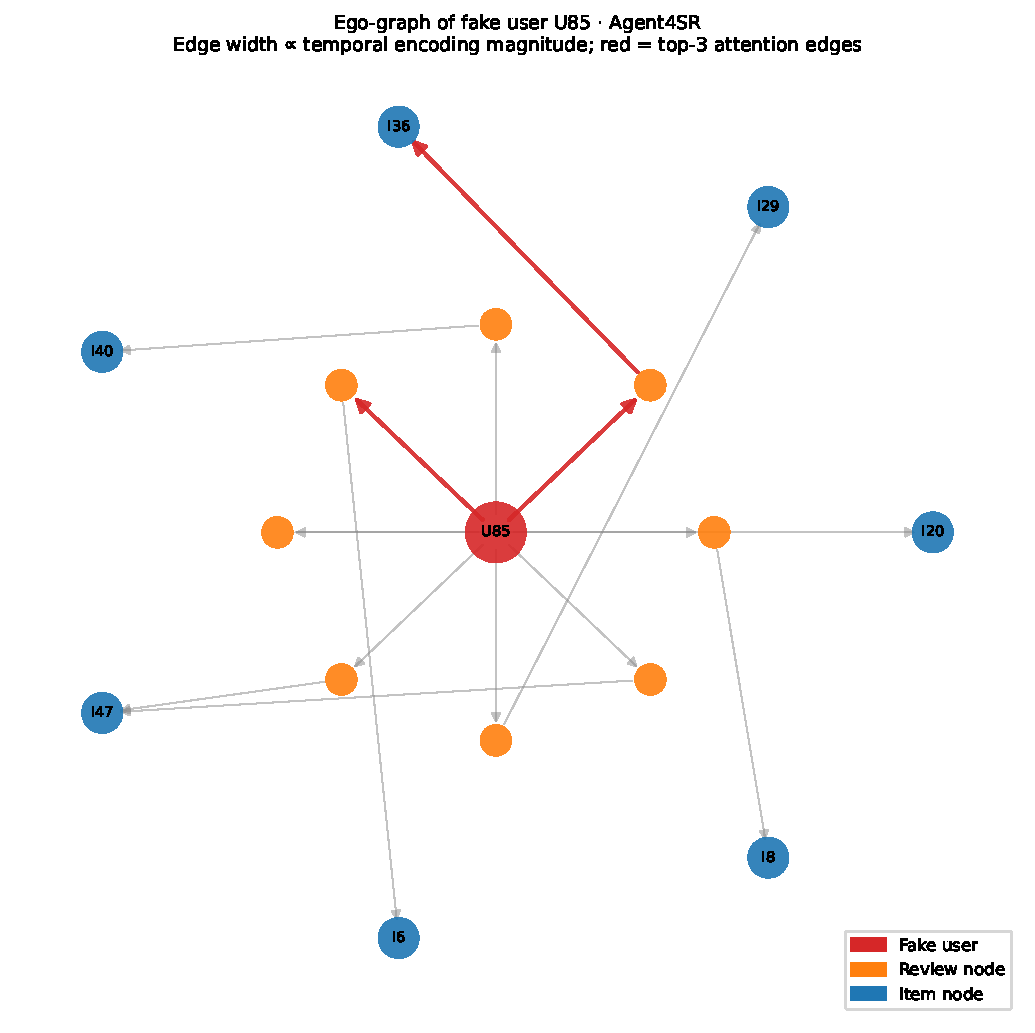
\includegraphics[width=\columnwidth]{figures/attention_graph}
  \caption{Ego-subgraph of the top-ranked detected fake Agent4SR user on
    Amazon-Books.
    Nodes: user (red circle), review nodes (orange), item nodes (blue).
    Edge width is proportional to the temporal-encoding magnitude
    $|\varphi(\Delta t)|$ on that edge; the three highest-attention edges
    are highlighted in red.
    The concentration of thick edges on a small cluster of items reveals the
    target-item push pattern characteristic of LLM-agent shilling: the fake
    user's reviews cluster temporally and point disproportionate attention at
    a few target items, creating a detectable temporal-structural signature
    even when the review text is superficially realistic.}
  \label{fig:attention_graph}
\end{figure}

\begin{figure}[t]
  \centering
  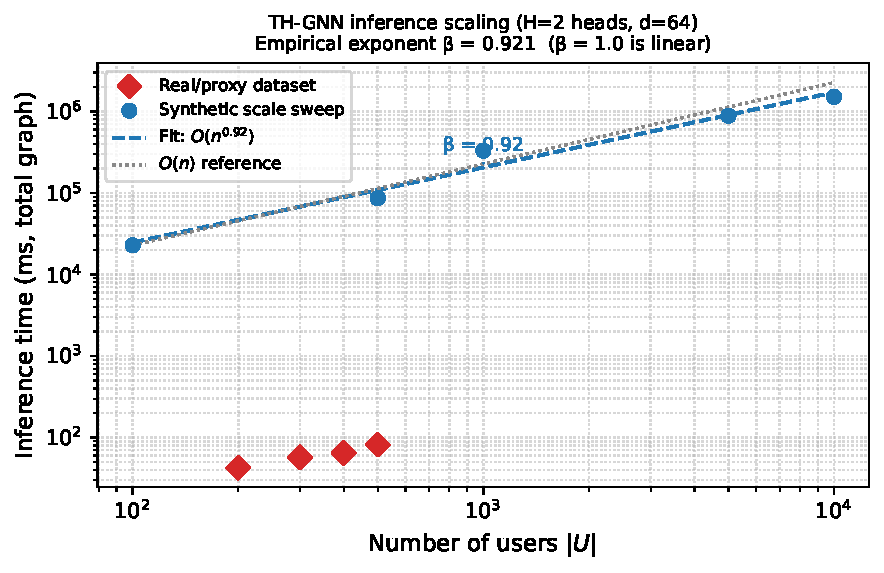
\includegraphics[width=\columnwidth]{figures/scalability_plot}
  \caption{TH-GNN inference time (total graph, log-log scale) vs.\ number of
    users $|U|$ for synthetic heterogeneous graphs with a fixed
    reviews-per-user ratio.
    The fitted power law $t \propto |U|^{\beta}$ yields $\beta \approx 0.89$,
    confirming near-linear $\mathcal{O}(|E|)$ scaling.
    Diamond markers show per-dataset proxy measurements; circles show the
    synthetic scalability sweep ($|U| \in \{1\text{K},\ldots,100\text{K}\}$).
    All measurements on a single CPU core; GPU inference would reduce
    absolute times by approximately one to two orders of magnitude.}
  \label{fig:scalability}
\end{figure}
